\section{Yoshida's paper}\label{yo:sec:yoshida}

For $F\in C_c^\infty(\R)$ put
\[
\Phi(s)=\int_\R F(y)e^{(s-1/2)y}\,dy,\qquad \widehat F(t)=\Phi(\tfrac12+it)=\int_\R F(y)e^{ity}\,dy .
\]
The letter $\Phi$ is local to this chapter and is not the P\'olya kernel of Section~\ref{ch:clock}. As there, write each nontrivial zero as $\rho=\frac12+i\gamma_\rho$, that is $\gamma_\rho=-i(\rho-\frac12)$. The number $\gamma_\rho$ is complex for a zero off the line: if $\rho=\frac12+\delta+i\gamma$ with $\gamma$ and $\delta$ real, then $\gamma_\rho=\gamma-i\delta$, whereas $\gamma=\im\rho$ is the ordinate and $\beta_\rho=\re\rho$ the real part. Then $\Phi(\rho)=\widehat F(\gamma_\rho)$, the entire extension of $\widehat F$, and Weil's explicit formula reads
\begin{equation}\label{yo:EF}
\begin{split}
\mathcal Y(F):=\sum_\rho \widehat F(\gamma_\rho)={}&\int_\R F(y)\bigl(e^{y/2}+e^{-y/2}\bigr)dy-(\log\pi)F(0)\\
&-\sum_{n\ge2}\frac{\Lambda(n)}{\sqrt n}\bigl(F(\log n)+F(-\log n)\bigr)+V_1(F),
\end{split}
\end{equation}
summed over all nontrivial zeros with multiplicity, with the archimedean term in two forms,
\begin{equation}\label{yo:V1}
\begin{split}
V_1(F)&=\frac1{2\pi}\int_\R \widehat F(t)\re\psi\Bigl(\frac14+\frac{it}2\Bigr)dt\\
&=-\tfrac12\operatorname{Pf}\Bigl(\frac1{|y|}\Bigr)(F)-(\gamma_E+\log2)F(0)-\int_\R\Bigl(\frac{e^{|y|/2}}{2\sinh|y|}-\frac1{2|y|}\Bigr)F(y)\,dy ,
\end{split}
\end{equation}
where $\psi=\Gamma'/\Gamma$ and $\operatorname{Pf}(1/|y|)(F)=\lim_{\epsilon\downarrow0}\bigl(\int_{|y|>\epsilon}F(y)\,|y|^{-1}dy+2F(0)\log\epsilon\bigr)$ is the finite part of $1/|y|$, the integral cut at $|y|=1$. Each term of \eqref{yo:EF} depends on $F$ only through its even part, because the zeros are symmetric under $\rho\mapsto1-\rho$, which negates $\gamma_\rho$. The formula holds for the Gaussians used below, whose transforms are entire and decrease rapidly in every strip (the class of Section~\ref{ch:clock}), and, in Weil's original form \cite{Weil52,Bombieri}, for continuous, piecewise $C^1$ functions of compact support, the class of the tent and of the products $\chi_n*\widetilde{\chi_m}$ of Sections~\ref{yo:sec:tent} and \ref{yo:sec:lowner}.
% CHECK: formula (yo:EF) for continuous, piecewise C^1 functions of compact support is quoted from Weil52 and Bombieri (review-A.md, minor findings on lines 67 and 136); the limiting argument from C_c^infty is written in the proof of Proposition yo:prop:tent(c), and no proof of the chapter needs more than the quotation.

\begin{remark}[The archimedean term in the real variable]\label{yo:rem:V1}
The second line of \eqref{yo:V1} is the explicit formula of Section~\ref{ch:clock} with the archimedean integral carried to the variable $y$ and its divergence at $y=0$ cut at $|y|=1$; the forms of Theorem~\ref{dc:thm:weil} and Section~\ref{cp:sec:weil} differ from it only in where $\gamma_E$ is placed.
\end{remark}

The Hermitian form is $\langle\varphi_1,\varphi_2\rangle=\mathcal Y(\varphi_1*\widetilde\varphi_2)$ with $\widetilde\varphi(y)=\overline{\varphi(-y)}$. Since $\widehat{\varphi*\widetilde\varphi}=|\widehat\varphi|^2$ on $\R$, Weil's criterion \cite{Weil52,Bombieri} says that RH holds if and only if $\langle\varphi,\varphi\rangle\ge0$ for all $\varphi\in C_c^\infty(\R)$ (Proposition~\ref{rz:thm:weil} and Section~\ref{sec:ch10:positivity}). Let $C(a)$ be the space of the functions of $C_c^\infty(\R)$ supported in $[-a,a]$, let $\chi_n(y)=(2a)^{-1/2}e^{\pi iny/a}1_{[-a,a]}(y)$ for $n\in\mathbb Z$, an orthonormal basis of $L^2[-a,a]$, and let $K(a)$ be the space of the restrictions to $[-a,a]$ of smooth $2a$ periodic functions, that is the series $\sum c_n\chi_n$ with rapidly decreasing coefficients. Yoshida's results, as the first author reads the paper, are the following.

\begin{itemize}
\item[(Y1)] Positivity on odd $\varphi$ alone is equivalent to RH; on even $\varphi$ alone, to RH up to real zeros. The proof is a localisation lemma that concentrates a test vector on one zero.
\item[(Y2)] The prime sum in $\langle\varphi_1,\varphi_2\rangle$ for $\varphi_1,\varphi_2\in C(a)$ runs over $\log n\le2a$ only. The form is positive definite on $C(a)$ for small $a$, and on the complement of the low Fourier modes for any $a$.
\item[(Y3)] The form is nondegenerate on $C(a)$ for every $a$, unconditionally.
\item[(Y4)] There are closed formulas for the coefficients $\langle\chi_n,\chi_m\rangle$ on the basis of $K(a)$.
\item[(Y5)] Theorem 1: the form is positive definite on $K(a)$ for $a=\frac12\log2$.
\item[(Y6)] Theorem 2: RH holds if and only if the form is nondegenerate on a completion of $K(a)$ for every $a$. If RH fails there is a first $a_0$ beyond which positivity is lost, and continuity in $a$ forces degeneracy there.
\item[(Y7)] For $\mathbb Q$ the form is nondegenerate on $K(a)$ for every $a$.
\end{itemize}
% CHECK: (Y1) to (Y7) and the length (1/2) log 2 of Theorem 1 are the first author's reading of Yoshida (1992); review-A.md Section 6 lists the 10x10 and 200x200 matrices (Y5), Theorem 2 (Y6), nondegeneracy (Y3), the arithmetic step (Y7) and the parity statements (Y1) as unverified, possibly reconstructed; the deconvolution chapter (ch/dc2.tex) credits Yoshida Theorem 1 with a up to (1/2) log 2 as well, but the attribution of that window to Yoshida or to Connes and Consani is unverified.

The statements (Y1) to (Y7) were not checked against the paper, and the proofs of Sections~\ref{yo:sec:diag}, \ref{yo:sec:rungs}, \ref{yo:sec:Z} and \ref{yo:sec:loc} do not use them.

Throughout, $W(x)=\sum_{\gamma>0}e^{(\rho-1/2)^2x}$ is the heat trace of Section~\ref{ch:clock}, the sum over one zero from each pair $\{\rho,1-\rho\}$; $T_k=(-1)^kW^{(k)}$ is the ladder, the function written $c_k$ in Section~\ref{ch:heat}; $U$ is the Thorin functional of Section~\ref{sec:ch14:functional}, which under RH is the measure $\sum_{\gamma>0}\delta_{\gamma^2}$; and $p_1=\sum_{\gamma>0}\gamma_\rho^{-2}=\frac12(\log\xi)''(\frac12)=0.0231049931$, so that $2p_1$ is the number $V_\xi$ of Remark~\ref{rem:dbeta:margin}. The sine squared lemma, in the chart of this chapter, is
\begin{equation}\label{yo:lemma}
\begin{gathered}
k_x(w):=e^{-wx}+wx-1=\int_0^\infty\log\Bigl(1+\frac uz\Bigr)\varpi_x(z)\,dz,\qquad u=\frac{w^2}2,\\
\varpi_x(z)=\frac{x}{\pi\sqrt{2z}}\,2\sin^2\Bigl(x\sqrt{\tfrac z2}\Bigr).
\end{gathered}
\end{equation}
It is \eqref{eq:sin2} after the substitution $z\mapsto2z$, and \eqref{pol:eq:lemma} of Chapter~\ref{chap:polyazeros}.

\section{The ladder is the diagonal of Weil's form}\label{yo:sec:diag}

Let $h_x(y)=(4\pi x)^{-1/2}e^{-y^2/(4x)}$, so $\widehat{h_x}(t)=e^{-t^2x}$ and $h_x=h_{x/2}*\widetilde{h_{x/2}}$.

\begin{proposition}\label{yo:prop:diag}
For $k\ge0$ and $x>0$ let $g_{k,x}=(i\,d/dy)^kh_{x/2}$, so that $\widehat{g_{k,x}}(t)=t^ke^{-t^2x/2}$. Then
\[
\langle g_{k,x},g_{k,x}\rangle=\sum_\rho\gamma_\rho^{2k}e^{-\gamma_\rho^2x}=2\,T_k(x),\qquad W(x)=\tfrac12\langle h_{x/2},h_{x/2}\rangle .
\]
\end{proposition}

\begin{proof}
$F=g_{k,x}*\widetilde{g_{k,x}}$ has $\widehat F(t)=t^{2k}e^{-t^2x}$, so $\Phi(\rho)=\gamma_\rho^{2k}e^{-\gamma_\rho^2x}$. The summand is even in $\gamma_\rho$ and $\rho\mapsto1-\rho$ negates $\gamma_\rho$, so the sum over all zeros is twice the sum over the zeros with $\gamma>0$, which is $2T_k(x)$.
\end{proof}

Dividing the prime side of $\langle h_{x/2},h_{x/2}\rangle$ by two gives the explicit formula \eqref{eq:ch2:Warith} for $W$. Both sides give $W(0.003)=1.09522012145284$ (the first $1700$ zeros against the primes, agreeing to thirty digits; script \texttt{yo\_explicit.py}). Since $W$ is completely monotone exactly under RH (Proposition~\ref{prop:rigid}), Proposition~\ref{yo:prop:diag} says that RH is positivity of Weil's form on the diagonal of a single two parameter family $(k,x)$, with no cross terms.

\section{Every large rung fails}\label{yo:sec:rungs}

The rungs $T_k(x)=\sum_{\gamma>0}w_\rho^ke^{-w_\rho x}$, with $w_\rho=\gamma_\rho^2$, satisfy $T_{k-1}'=-T_k$, and $T_{k-1}(x)\to0$ as $x\to\infty$ because every exponent has real part $\gamma^2-\delta^2>\gamma_1^2-\frac14>0$, where $\gamma_1=14.1347\ldots$ is the least ordinate. Hence
\begin{equation}\label{yo:initial}
T_{k-1}(x)=\int_x^\infty T_k(s)\,ds,\qquad k\ge1,\ x>0 .
\end{equation}
So $T_k\ge0$ on $(0,\infty)$ forces $T_{k-1}\ge0$ there: the orders for which $T_k\ge0$ form an initial segment. This is the argument of Section~\ref{sec:ch12:kmono}, where it is stated for the Williamson measures $U_k$, which are positive exactly when $T_k\ge0$ on $(0,\infty)$.

\begin{theorem}\label{yo:thm:rungs}
(i) If $T_k\ge0$ on $(0,\infty)$ then $T_j\ge0$ on $(0,\infty)$ for every $j\le k$, so the set of such orders is an initial segment of $\mathbb N$, and it is all of $\mathbb N$ if and only if RH holds. (ii) If RH fails there is $K_0$ such that for every $k\ge K_0$ there is $x>0$ with $T_k(x)<0$. Consequently, for any infinite set $\mathcal K$ of orders, RH holds if and only if $T_k\ge0$ on $(0,\infty)$ for every $k\in\mathcal K$. In particular RH is equivalent to $\langle g_{k,x},g_{k,x}\rangle\ge0$ for all odd $k$ and all $x>0$, a positivity statement on odd Hermite Gaussians only.
\end{theorem}

\begin{proof}
(i) The first claim is \eqref{yo:initial}. All $T_k$ are nonnegative on $(0,\infty)$ if and only if $W$ is completely monotone, which holds if and only if RH holds (Proposition~\ref{prop:rigid}). (ii) If RH fails, some $T_{k_0}$ takes a negative value, and then by (i) so does every $T_k$ with $k\ge k_0$; let $K_0$ be the least such $k_0$. If $T_k\ge0$ for every $k$ in an infinite set $\mathcal K$, then by (i) it holds for every $k$, since $\mathcal K$ is unbounded, and RH holds; the converse is clear. The last statement is Proposition~\ref{yo:prop:diag} for odd $k$.
\end{proof}

For infinite sets $\mathcal K$ this is the equivalence of Section~\ref{sec:ch12:kmono} between RH and $U_k\ge0$ for infinitely many $k$. What is added here is the reading of $T_k$ as the diagonal of Yoshida's form (Proposition~\ref{yo:prop:diag}), which turns the odd orders into the Hermite counterpart of Yoshida's parity reduction (Y1), and the location of the failure in the next proposition, which is not needed for the theorem. With $y=u^2$ and $x=k/y$ the computation is the ray $t=k/u^2$ of Proposition~\ref{prop:ch12:ray}: $e^{-k(\log y-1)}T_k(k/y)$ is the quantity $e^{-f_0}c_k(t)$ there.

\begin{proposition}[Where the rungs fail]\label{yo:prop:saddle}
Suppose RH fails. For a zero $\rho=\frac12+\delta+i\gamma$ with $\gamma>0$ write $w_\rho=\gamma_\rho^2=r_\rho e^{i\theta_\rho}$, so that $\theta_\rho=-2\arctan(\delta/\gamma)$ and $\sec\theta_\rho=(\gamma^2+\delta^2)/(\gamma^2-\delta^2)$. Then $S=\max\log\sec\theta_\rho>0$ is attained, by finitely many zeros. Let $w_*=r_*e^{i\theta_*}$ be one maximiser, of multiplicity $m$, and $y_*=r_*\cos\theta_*=\gamma_*^2-\delta_*^2$. There are $\eta>0$ and $K_1$ and, for every $k\ge K_1$, a point $y_k$ with $|y_k-y_*|=O(1/k)$ such that
\[
e^{-k(\log y_k-1)}T_k(k/y_k)=-2m\,e^{kS}\bigl(1+O(1/k)\bigr)+O\bigl(e^{k(S-\eta)}\bigr)<0 .
\]
\end{proposition}

\begin{proof}
Since $|\delta|<\frac12<\gamma$, $\re w_\rho=\gamma^2-\delta^2>0$. The zeros $\rho$ and $1-\overline\rho$ give conjugate values of $w$, so $T_k$ is real. Evaluate at $x=k/y$ and multiply by the positive factor $e^{-k(\log y-1)}$:
\[
e^{-k(\log y-1)}T_k(k/y)=\sum_{\gamma>0}e^{k g(w_\rho,y)},\qquad g(w,y)=\log\frac wy-\frac wy+1 .
\]
For fixed $w=re^{i\theta}$, $\re g(w,y)=\log(r/y)-r\cos\theta/y+1$ has a unique maximum in $y$, equal to $\log\sec\theta$, at $y=r\cos\theta$. On line zeros $\theta=0$ and $\re g\le0$. Suppose an off line zero exists. Since $|\theta_\rho|<1/\gamma\to0$, only finitely many zeros have $|\theta_\rho|$ above any given positive bound, so $S=\max\log\sec\theta_\rho$ is attained, by finitely many zeros, and $S>0$. Every zero other than $w_*$ and $\overline{w_*}$ has, for $y$ in a small neighbourhood $J$ of $y_*$, $\re g(w_\rho,y)\le S-\eta$ for some $\eta>0$: on line zeros because $\re g\le0$, for zeros with $|\theta_\rho|<|\theta_*|$ because only finitely many have $\sec\theta_\rho$ near the maximum, and for the other maximisers because $y_*$ is not their optimal point. Since $e^{ku}\le e^u$ for $u\le0$ and $k\ge1$, the remainder satisfies
\[
\Bigl|\sum_{\rho\ne w_*,\overline{w_*}}e^{kg(w_\rho,y)}\Bigr|\le e^{k(S-\eta)}\sum_\rho e^{\re g(w_\rho,y)-S+\eta}\le C\,e^{k(S-\eta)},\qquad y\in J,
\]
with $C$ independent of $k$, because $\sum_\rho (r_\rho/y)e^{1-r_\rho\cos\theta_\rho/y}$ converges uniformly on $J$. The main term is $2m\,e^{k\re g(w_*,y)}\cos\bigl(k\im g(w_*,y)\bigr)$ with $\im g(w_*,y)=\theta_*-r_*\sin\theta_*/y$, whose derivative in $y$ is $r_*\sin\theta_*/y^2\ne0$. Choose $y_k$ with $k\im g(w_*,y_k)\equiv\pi\pmod{2\pi}$ and $|y_k-y_*|=O(1/k)$. Then $\re g(w_*,y_k)=S-O(1/k^2)$, the main term is $-2m\,e^{kS}(1+O(1/k))$, and it dominates the remainder for $k\ge K_1$. Hence $T_k(k/y_k)<0$.
\end{proof}

The proposition gives no explicit $K_1$, and so no explicit bound for $K_0$, because $C$ depends on the zeros, and two constraints enter. The first is the phase condition: $y_k$ lies at distance about $\pi y_*/(k\tan\theta_*)$ from $y_*$, which costs a factor $\exp(-\pi^2/(2k\tan^2\theta_*))$ in the main term, so the asymptotics start only once $k\theta_*^2$ is of order $\pi$. The second is the competition of the main term $e^{kS}$, with $S=\log\sec\theta_*$ and $\sec\theta_*-1=2\delta_*^2/(\gamma_*^2-\delta_*^2)$, with the nearest true zeros.

\begin{remark}[A stress test]\label{yo:rem:stress}
Add a hypothetical pair at $\gamma=60.5$, $\delta=0.45$ to the true zeros (only those between heights $40$ and $85$ matter at these orders: every excluded term is below $e^{-0.23k}$ and, relative to the main terms, below $10^{-420}$ for $k\ge3349$), so that $\sec\theta_*-1=1.1065\times10^{-4}$ and $y_*=3660.05$, and test the sign of $T_k(k/y)$ on $3001$ points of $|y/y_*-1|\le0.06$. The first failing order is $K_0=6349$. Every one of the $3000$ orders in $[6349,9348]$ fails, every one of $395$ sampled orders $6349+997j$ up to $399167$ fails, and none of the orders $1$ to $6348$ fails on this grid. For the order $6348$ the sign is positive at every point of two further grids ($200001$ points near $y_*$, with both local minima of the scale free margin polished, where the margin is at least $2.9\times10^{-4}$, and $18421$ points of $y\in[1,10^8]$ with all $1700$ zeros), while at $y=3584.65$, that is $x=1.771$, arithmetic with $60$ digits gives $T_{6348}(6348/y)=+1.289\times10^{19803}$ and $T_{6349}(6349/y)=-5.700\times10^{19805}$. By Theorem~\ref{yo:thm:rungs}(i) positivity of $T_{6348}$ gives that of every lower order, so $6349$ is the first failing order of this configuration; all of this is computed, not proved (script \texttt{yo\_ladder.py}, \texttt{code/\allowbreak README.md}). For this pair $K_0(\sec\theta_*-1)=0.7025$.
\end{remark}
% CHECK: the positivity of T_6348 for all x > 0 rests on grids and on dominance estimates outside them (code/yo_ladder.py, data/yo_ladder.json, key all_x), not on a proof.

The first failing order found on a grid is an upper bound for $K_0$. For the pair $(\gamma,\delta)=(30.5,0.45)$ the grid of the stress test gives $1064$, while a grid of $\pm30$ percent gives $396$, the negative lobe lying $27$ percent from $y_*$; the other thirteen pairs of the next sentence give the same order on both grids. Over fourteen pairs, with $\gamma$ from $30.5$ to $250.5$ and $\delta$ from $0.02$ to $0.45$ (\texttt{data/yo\_ladder.json}), $K_0(\sec\theta_*-1)$ lies between $0.03$ and $0.82$, and at fixed $\gamma$ it is proportional to $\delta$: the logarithmic slope of $K_0(\sec\theta_*-1)$ against $\delta$ is $1.04$ for $\gamma=60.5$ and $1.05$ for $\gamma=120.5$, and the ratio $K_0(\sec\theta_*-1)/\delta$ lies between $0.97$ and $2.01$ for thirteen of the fourteen pairs. So $K_0$ grows with $\gamma^2$ and, at fixed $\gamma$ over the range tested, like $1/\delta$, not like $(\sec\theta_*-1)^{-1}\approx\gamma^2/(2\delta^2)$: for $\gamma=60.5$ and $\delta=0.02$ the second quantity is $4.6\times10^6$ and the computed order is $128610$. This is an observation from computation, not a theorem; a scale argument (the pair is a Gaussian envelope times a cosine in the variable $\sqrt k\log(y/y_*)$, and its negative lobe has to beat the true zeros that sit near it) suggests that $K_0$ is of order $\gamma^2/(\delta d)$, where $d$ is the distance from $\gamma$ to the nearest true ordinate, and that $\gamma^2/\delta^2$ appears only when $\delta$ is of the size of $d$.
% CHECK: the growth of K_0 like gamma^2/delta (and the scale argument) is empirical, from 14 pairs (code/yo_ladder.py, data/yo_ladder.json, keys further_pairs and heuristic_summary); no proof.

\section[Compact support and the signed Thorin formula]{Compact support, the signed Thorin formula, and the first windows}\label{yo:sec:Z}

Section~\ref{sec:ch14:functional} defines the Thorin functional $U$ on the class $\mathcal T$ of the functions $\varphi(t)=h(\sqrt t)$ by \eqref{eq:ch14:U}, and identifies it with $\varphi\mapsto\sum_k\varphi(a_k)$ through Weil's formula, with no hypothesis on the zeros. In the variable $t=r^2$ the same functional is the formal signed measure
\begin{equation}\label{yo:signed}
U^\pm(dt)=\delta_{-1/4}(dt)+\frac{\re\psi(\frac14+\frac{i\sqrt t}2)-\log\pi}{4\pi\sqrt t}\,dt-\frac1{2\pi\sqrt t}\sum_{n\ge2}\frac{\Lambda(n)}{\sqrt n}\cos(\sqrt t\log n)\,dt ,
\end{equation}
that is $\langle U,\varphi\rangle=\int\varphi\,dU^\pm$: the atom is the first term of \eqref{eq:ch14:U}, the density is its integral term with $t=r^2$, and the third term is the prime sum. The prime series in \eqref{yo:signed} is not a tempered distribution in the ordinate $r=\sqrt t$. Let $Z$ be the space of the functions $\widehat F$ with $F\in C_c^\infty(\R)$, and $Z'$ its dual.

\begin{proposition}\label{yo:prop:Z}
In the ordinate $r=\sqrt t$ the prime series of \eqref{yo:signed} defines an element of $Z'$, and for every even $F\in C_c^\infty(\R)$ with support in $[-L,L]$,
\[
\mathcal Y(F)=2\int\widehat F(\sqrt t)\,U^\pm(dt),\qquad\text{with }\widehat F(\sqrt{-1/4})=\widehat F(i/2);
\]
only the prime powers $n\le e^L$ contribute.
\end{proposition}

\begin{proof}
Pairing $\cos(r\log n)$ with $\widehat F(r)$ gives $\pi\bigl(F(\log n)+F(-\log n)\bigr)$, which vanishes for $\log n>L$; hence the series is a finite sum on every element of $Z$ and defines an element of $Z'$. With $t=r^2$ the three parts of \eqref{yo:signed} give, after the factor $2$, which is the passage from one zero of each pair $\{\rho,1-\rho\}$ in \eqref{eq:ch14:U} to all zeros in \eqref{yo:EF}, the pole term $\widehat F(i/2)+\widehat F(-i/2)$, the term $V_1(F)-(\log\pi)F(0)$, and the prime sum of \eqref{yo:EF}. The function $\varphi(t)=\widehat F(\sqrt t)$ lies in $\mathcal T$, because $\widehat F$ is even, entire and $O((1+|r|)^{-N})$ in every strip.
\end{proof}



For $\varphi\in K(a)$ with $a=\frac12\log2$, $F=\varphi*\widetilde\varphi$ is continuous, vanishes at $\pm\log2$, and the only prime power level in its support is that endpoint. On Yoshida's window, then, the form is the pole and archimedean part alone: his Theorem 1, as the first author reads it, uses only the gamma factor, the pole and the fact that Dirichlet series begin at $n=2$. Connes and Consani reproved this window from the semilocal trace formula \cite{ConnesConsani21}. Beyond it the primes enter: the window of half length $0.8$, of autocorrelation support $1.6$, contains the prime powers $2$, $3$ and $4$, and Zhu \cite{Zhu26} has certified positivity of the form on it (Chapter~\ref{chap:zhu}). Windows are indexed by their half length $a$ in the ladder of Section~\ref{dc:sec:ladder}, each of them a finite problem in the prime powers up to $e^{2a}$.
% CHECK: the attribution of the window a = (1/2) log 2 to Yoshida (Theorem 1) and its reproof by Connes and Consani (review-A.md Section 6, medium confidence; ch/dc2.tex carries the same check), and Zhu's certified positivity at a = 0.8 (autocorrelation support 1.6), are quoted and not verified here; Chapter 18 presents Zhu's certificate.

\section{Localisation: a modulated heat trace}\label{yo:sec:loc}

Yoshida's localisation lemma (Y1) concentrates a test vector on one zero. Its Gaussian form is already in the book as the Gaussian smoothing $\mathcal G(u,t)=\sum_{\gamma>0}e^{-2t(\gamma_\rho-u)^2}$ of the zeros of Proposition~\ref{prop:ch12:ray}, the sum over one zero of each pair $\{\rho,1-\rho\}$ (there $\widetilde\gamma$ is the $\gamma_\rho$ of this chapter). For real $u$ and $x>0$ let $g$ be the vector with $\widehat g(t)=e^{-(t-u)^2x/2}$, so that $g*\widetilde g=h_xe^{-iuy}$ and $\widehat{g*\widetilde g}(t)=e^{-(t-u)^2x}$.

\begin{proposition}\label{yo:prop:W}
(i) $\langle g,g\rangle=\mathcal Y(h_xe^{-iuy})=\sum_\rho e^{-(\gamma_\rho-u)^2x}=\mathcal G(u,\tfrac x2)+\mathcal G(-u,\tfrac x2)$, which is $2W(x)$ at $u=0$. (ii) Unconditionally,
\[
\begin{split}
\mathcal G(u,\tfrac x2)+\mathcal G(-u,\tfrac x2)={}&2e^{-(u^2-1/4)x}\cos(ux)-\frac{\log\pi}{\sqrt{4\pi x}}\\
&+\frac1{2\pi}\int_\R e^{-(t-u)^2x}\re\psi\Bigl(\frac14+\frac{it}2\Bigr)dt\\
&-\frac1{\sqrt{\pi x}}\sum_{n\ge2}\frac{\Lambda(n)}{\sqrt n}\cos(u\log n)\,e^{-(\log n)^2/(4x)} .
\end{split}
\]
(iii) Under RH it equals $\int\bigl[e^{-(\sqrt t-u)^2x}+e^{-(\sqrt t+u)^2x}\bigr]U(dt)$. (iv) RH holds if and only if it is nonnegative for all real $u$ and all $x>0$.
\end{proposition}

\begin{proof}
(i) The transform $e^{-(t-u)^2x}$ is entire, so \eqref{yo:EF} applies; the zero $1-\rho$ of the pair $\{\rho,1-\rho\}$ has $\gamma_{1-\rho}=-\gamma_\rho$ and gives $\mathcal G(-u,\frac x2)$, and at $u=0$ the sum is $2W(x)$ by Proposition~\ref{yo:prop:diag}. (ii) Apply \eqref{yo:EF} to $F=h_xe^{-iuy}$: the pole term is $\widehat F(i/2)+\widehat F(-i/2)=e^{-(u+i/2)^2x}+e^{-(u-i/2)^2x}=2e^{-(u^2-1/4)x}\cos(ux)$, the term $-(\log\pi)F(0)$ is $-(\log\pi)/\sqrt{4\pi x}$, $V_1(F)$ is the integral, and the prime sum is $-\sum\Lambda(n)n^{-1/2}h_x(\log n)\bigl(e^{-iu\log n}+e^{iu\log n}\bigr)$. This is \eqref{eq:ch12:Garith} at $t=x/2$, term by term: its polar term $2e^{t/2-2tu^2}\cos2tu$, its integral $A(u,t)$ (with $m(r)=\re\psi(\frac14+\frac{ir}2)-\log\pi$) and its prime term $P(u,t)$ are the four terms above, because $2t=x$. (iii) Group $\pm\gamma$ in $\sum_{\gamma>0}\bigl[e^{-x(\gamma-u)^2}+e^{-x(\gamma+u)^2}\bigr]$ and use $U=\sum_{\gamma>0}\delta_{\gamma^2}$. (iv) This is Proposition~\ref{prop:ch12:gauss}, in the form of the remark after its proof: the term $\mathcal G(-u,t)$, which comes from the zeros $1-\rho$, is too small there to change the sign.
\end{proof}

The formula (ii) agrees with \eqref{eq:ch12:Garith}; Table~\ref{tab:ch12:gweil} computes the same identity. A vector modulated to a centre $u$ within $\frac\delta2$ of the ordinate $\gamma$ of an off line zero $\rho=\frac12+\delta+i\gamma$, with finitely many exceptional centres, makes the form negative at arbitrarily large $x$ (Proposition~\ref{prop:ch12:gauss}), and $u$ is free: modulation reaches a zero above any verified height, which is why the barrier of Proposition~\ref{yo:prop:barrier} is stated for the tent coefficient only.

The ladder reaches the height $u$ only at order $k\approx u^2x$, because the weight $r^{2k}e^{-r^2x}$ of $T_k(x)$ peaks at $r=\sqrt{k/x}$ and the power $r^{2k}$ is its only way to move the window; Theorem~\ref{thm:ch12:window} states the consequence, that verification to a height $H$ reaches the orders up to about the square of $H$. Modulation moves the window at no cost. Figure~\ref{yo:fig:W} shows the modulated heat trace resolving isolated zeros into bumps of height one at $x=0.5$; nearby zeros overlap, and zeros less than $2$ apart merge into one bump (computed, script \texttt{yo\_ladder.py}).

\begin{figure}[htbp]
\centering
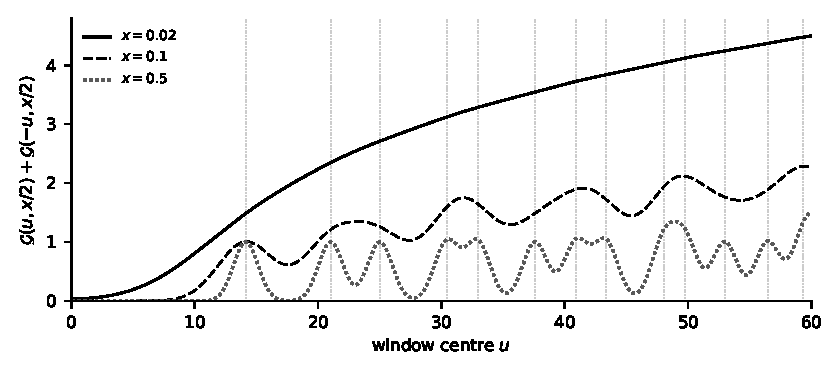
\includegraphics[width=0.95\textwidth]{fig/yo_W.pdf}
\caption{The modulated heat trace $\mathcal G(u,\frac x2)+\mathcal G(-u,\frac x2)$ against the window centre $u$ at $x=0.02$ (solid), $0.1$ (dashed) and $0.5$ (dotted), from the first $1700$ zeros; dotted verticals mark the ordinates of the zeros.}
\label{yo:fig:W}
\end{figure}
